\chapter{Gabor Wavelet and AdaBoost}
\label{ch:gaboradaboost}
This chapter presents the fundamentals of the Gabor-Boosting algorithm: Gabor wavelets and AdaBoost. \mbox{Section} \ref{sec:faceveri} discusses the Gabor wavelets and how face images are represented by Gabor wavelet features. In \mbox{Section} \ref{sec:faceveri:adaboost}, the AdaBoost algorithm is presented, and the principle of constructing the ``strong'' AdaBoost ensemble classifier, is discussed.
\section{Gabor Wavelets}
\label{sec:faceveri}
A 2-D Gabor filter is a linear filter whose kernel is similar to the 2-D receptive profiles of the mammalian cortical simple cells \cite{Jones1987}. A 2-D Gabor kernel is a 2-D Gaussian function multiplied by a 2-D harmonic function. Generally, a harmonic function is a Fourier basis function. Especially, in a 2-D Gabor kernel it is a sinusoidally modulated function, in a form of complex exponential function. The Gaussian function varies in dilation and the harmonic function varies in rotation and frequency, so that a group of 2-D Gabor filters can be formed into 2-D Gabor wavelets. Gabor wavelets capture local structure corresponding to spatial frequency, \textit{i.e.}, scale, spatial localisation (coordinates), and orientation selectivity.

Gabor wavelets are used to extract facial information from face images. \mbox{Section} \ref{sec:backgoundGabor} gives the background study on Gabor wavelets. The definition of Gabor wavelet is given in \mbox{Section} \ref{sec:definGabor}. \mbox{Section} \ref{sec:gaborwavelettransform} illustrates the Gabor wavelet transform. \mbox{Section} \ref{sec:gaborwaveletfeature} presents the representatives of face images - Gabor wavelet features.
\subsection{Background of Gabor Wavelets}
\label{sec:backgoundGabor}
2-D Gabor wavelets are widely adopted as a feature extraction approach in texture segmentation \cite{Dunn1994,Dunn1995,Jain1991,Teuner1995}, iris recognition \cite{Daugman1988}, face recognition \cite{Wiskott1997,Wiskott1999}, face expression recognition \cite{Hong1998,Lyons1999,Zhang1998}, and image retrieval \cite{Manjunath1996}.

When Gabor filters are applied on computer vision or image processing tasks, the one biggest problem is how to select the appropriate Gabor filters, \textit{i.e.}, finding appropriate parameters for Gabor filters. The parametric characterisation has been studied extensively and different types of schemes have emerged. In \cite{Dunn1994}, 2-D Gabor filters transform different texture into detectable filter-output discontinuities at texture boundaries. Gabor filter output is modeled as Rician random variables \cite{Dunn1994}. A decision algorithm for selecting optimal filter parameters based on the Rician model is developed by Dunn and Higgins \cite{Dunn1995}. In \cite{Jain1991}, a bank of Gabor filters is characterised as uniformly covering the spatial-frequency domain, and a filter selection scheme is presented based on minimal ``energy'' loss in reconstructed images from the filtered images. Teuner \textit{et al.} \cite{Teuner1995} choose parameters of Gabor filters based on the analysis of spectral feature contrasts obtained from iterations of pyramidal Gabor transforms. The work benefit from not needing prior knowledge of the texture image which means the segmentation processing is unsupervised. Since these parametrization solutions are all to choose optimal frequency or orientation of Gabor filter, an alternative wavelet scenario is proposed to bypass the optimisation. 

A 2-D Gabor wavelet model with multi-scale and multi-orientation is originally proposed by Daugman \cite{Daugman1985, Daugman1988} for biometric research. In \cite{Daugman1988}, by using a three-lay neural network, a nonorthogonal 2-D Gabor representation is generalised. Daugman also has applied his 2-D Gabor wavelet model on human iris recognition.  In \cite{Daugman1993}, the visible texture of the human iris is transformed as a sequence of multi-scale 2-D Gabor wavelet digits. Lades \textit{et al.} \cite{Lades1993} has applied Gabor wavelets for face recognition using the Dynamic Link Architecture (DLA) framework. The DLA starts by computing Gabor wavelets, and then it performs a flexible template comparison between resulting image decompositions using graph-matching. Wiskott \textit{et al.} \cite{Wiskott1997,Wiskott1999} have extended on DLA by developing a Gabor wavelet based Elastic Bunch Graph Matching (EBGM) to label and recognise faces. Faces are represented by labelled graphs using Gabor wavelet transform. The labelled graphs consist of nodes and edges which are positioned by elastic bunch graph matching processing for comparing similarities. The testing is done on the FERET database \cite{Phillips2000} showing a high recognition rate for frontal face images. Liu and Wechsler \cite{Liu2002} applied the Enhanced Fisher linear discriminant Model (EFM) to an augmented Gabor feature vector \cite{Liu2001} derived from the Gabor wavelet representation of face images. Liu \cite{Liu2004} also presents a Gabor-based kernel Principal Component Analysis (PCA) method by integrating Gabor wavelet representation and the kernel PCA for recognition.  Fan \textit{et al.} \cite{Fan2004} combined Gabor wavelet and Null space-based Linear Discriminate Analysis (LDA) simultaneously on each orientations for generating feature vectors.

In analysis of facial expression, the recognition is to analyse the relationship between the movements made by facial features, such as eyebrows, eyes and mouth. These facial features can be defined as point-based visual properties of facial expressions. Hong \textit{et al.} \cite{Hong1998} use Gabor wavelets of five frequencies and eight orientations to define a ``big'' General Face Knowledge (GFK) with $50$ nodes\footnote{The nodes are landmark points on human faces.} on a face, and a ``small'' $16$-node GFK with three frequencies and four orientations. The method which fits these nodes with face image is the elastic graph matching proposed by Wiskott \textit{et al.} \cite{Wiskott1997,Wiskott1999} in face recognition. Zhang \textit{et al.} \cite{Zhang1998} use $34$ facial points for which a set of Gabor wavelet coefficients, the Gabor wavelets with three frequencies and six orientations have been utilised. Lyons \textit{et al.} \cite{Lyons1999} use a fiducial grid of $34$ nodes and apply wavelets of five frequencies and six orientations.


\subsection{The Definition of Gabor Wavelets}
\label{sec:definGabor}
Gabor wavelets are introduced to image analysis due to their biological relevance and computational properties \cite{Jones1987}. A Gabor wavelet \cite{Daugman1988} (sometimes, called Gabor Kernel or Gabor Elemental Function \cite{Dunn1994}) is defined as 
\begin{equation}\label{eq:kernel}
\psi_{\mu,\nu}(z)=\frac{\|{k_{\mu,\nu}}\| ^ {2}}{\sigma ^{2}}e^{-\frac{\|{k_{\mu,\nu}}\|^ {2}\|z\|^{2}}{2\sigma ^{2}}}\lbrack{e^{ik_{\mu,\nu} z}-e^{-\frac{\sigma^2}{2}}}\rbrack
\end{equation}
where $z=(x,y)$ indicates a point with $x$, the horizontal coordinate and $y$, the vertical coordinate. The parameters $\mu$ and $\nu$ define the angular orientation and the spatial frequency of the Gabor kernel. In \mbox{Equation} \ref{eq:kernel}, the spatial frequency modulates the size of the 2-D discrete Gabor kernel, so that $\nu$ also determines the scale of kernel. The operator $\|\cdot\|$ denotes the norm operator. The parameter $\sigma$ is the standard deviation of Gaussian window in the kernel. The wave vector $k_{\mu,\nu}$ is defined as
\begin{equation}\label{eq:wavevector}
k_{\mu,\nu}=k_{\nu}e^{i\phi_{\mu}}
\end{equation}
where $k_{\nu}=\frac{k_{max}}{f^{\nu}}$ and $\phi_{\mu}=\frac{\pi\mu}{8}$ if eight different orientations have been chosen. $k_{max}$ is the maximum frequency, and $f$ is the spatial factor between
kernels in the frequency domain.
\subsubsection{Wavelets}
Gabor kernels in \mbox{Equation} (\ref{eq:kernel}) are all self-similar since they are generated from one kernel (from one mother wavelet) by dilation and rotation via the wave vector $k_{\mu,\nu}$. Each kernel is a product of a Gaussian envelope formulated in the \mbox{Equation}
\begin{equation}\label{eq:gaussian}
 \frac{\|{k_{\mu,\nu}}\| ^ {2}}{\sigma ^{2}}e^{-\frac{\|{k_{\mu,\nu}}\|^ {2}\|z\|^{2}}{2\sigma ^{2}}}\
\end{equation}
and a complex plane wave $e^{ik_{\mu,\nu} z}$. The complex wave determines the oscillatory part of the kernel. The term $-e^{-\frac{\sigma^2}{2}}$ compensates for the Disparity Compensated (DC) value which makes the kernel DC-free. DC-free \cite{Krueger2001} is a wavelet terminology that ensures wavelets do not lose any generality such that there is no minimal energy loss when images are reconstructed by the wavelets. The effect of the DC term becomes negligible when the parameter $\sigma$, which determines the ratio of the Gaussian window width to wavelength, is a sufficiently large value.

\subsubsection{Parametrization}
In this thesis, five different scales and eight orientations of Gabor wavelets are used, i.e., $\nu\in\{-1,\ldots,3\}$, and $\mu\in\{0,\ldots,7\}$. Since images used in this thesis are smaller than the images with $128\times 128$ size used in \cite{Wiskott1997,Wiskott1999}, the scale range is from $-1$ to $3$ rather than from $0$ to $4$. The eight orientations in radian are from $0$ to $7\pi/8$ with a $\pi/8$ interval. Gabor wavelets are modulated by a Gaussian envelope function with relative width $\sigma=2\pi$. The maximum frequency is $k_{max}=\frac{\pi}{2}$, and the factor $f=\sqrt{2}$. These parameters are chosen according to previous findings \cite{Wiskott1999,Liu2004}. The kernels exhibit desirable characteristics of spatial frequency, spatial locality, and orientation selectivity. 

\subsubsection{Complex Gabor}
Gabor kernel is a product of a Gaussian and a complex plane wave with real and imaginary parts, also called even and odd. The \mbox{Equation} \ref{eq:kernel} is separated into real and imaginary parts, so that the real part is
\begin{equation}\label{eq:real}
\frac{k_{\nu}^2}{\sigma^2}e^{-{\frac{\|z\|^2 k_{\nu}^2}{2\sigma^2}}} \{\cos(k_{\nu}\cos(\phi_{\mu})x+k_{\nu}\sin(\phi_{\mu})y)-e^-{\frac{\sigma^2}{2}}\}
\end{equation}
and the imaginary part becomes
\begin{equation}\label{eq:imag}
\frac{k_{\nu}^2}{\sigma^2} e^-{\frac{\|z\|^2 k_{\nu}^2}{2\sigma^2}} \sin(k_{\nu}\cos(\phi_{\mu})x+k_{\nu}\sin(\phi_{\mu})y)
\end{equation}
The real part and the imaginary part of $40$ Gabor wavelets are shown in \mbox{Figure} \ref{fig:realgabor} and \mbox{Figure} \ref{fig:imaggabor} respectively.
\begin{figure}[ht]
 \begin{center}
 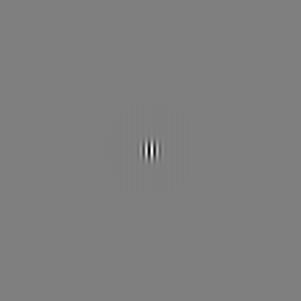
\includegraphics[width=\columnwidth/9]{ch4/figures/rGabor0_0.jpg}
 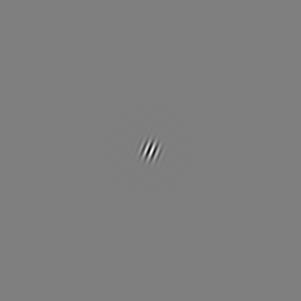
\includegraphics[width=\columnwidth/9]{ch4/figures/rGabor0_1.jpg}
 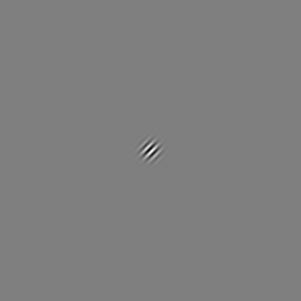
\includegraphics[width=\columnwidth/9]{ch4/figures/rGabor0_2.jpg}
 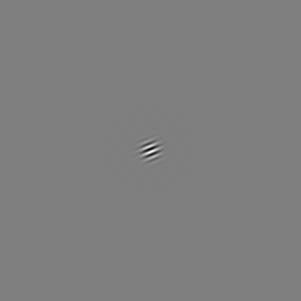
\includegraphics[width=\columnwidth/9]{ch4/figures/rGabor0_3.jpg}
 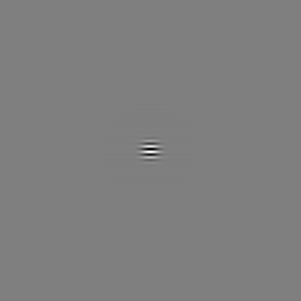
\includegraphics[width=\columnwidth/9]{ch4/figures/rGabor0_4.jpg}
 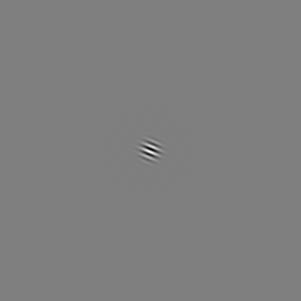
\includegraphics[width=\columnwidth/9]{ch4/figures/rGabor0_5.jpg}
 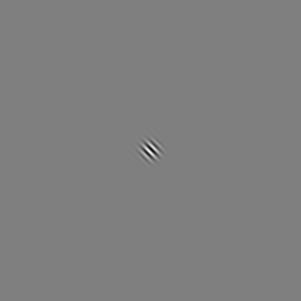
\includegraphics[width=\columnwidth/9]{ch4/figures/rGabor0_6.jpg}
 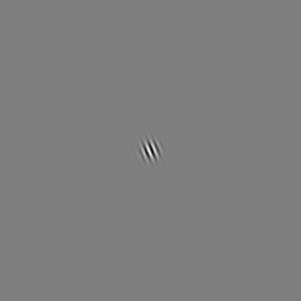
\includegraphics[width=\columnwidth/9]{ch4/figures/rGabor0_7.jpg}\\
 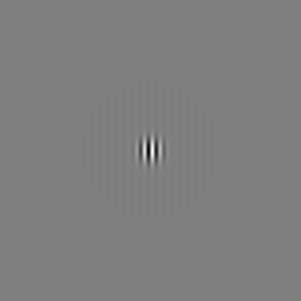
\includegraphics[width=\columnwidth/9]{ch4/figures/rGabor1_0.jpg}
 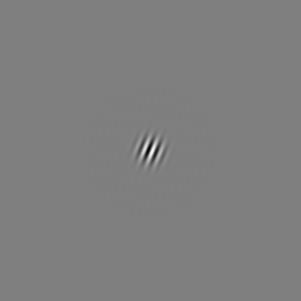
\includegraphics[width=\columnwidth/9]{ch4/figures/rGabor1_1.jpg}
 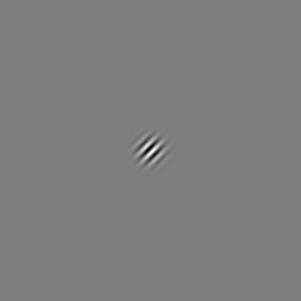
\includegraphics[width=\columnwidth/9]{ch4/figures/rGabor1_2.jpg}
 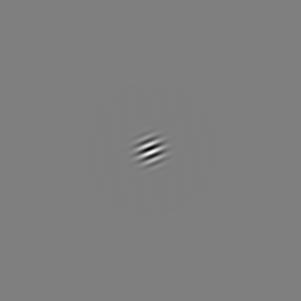
\includegraphics[width=\columnwidth/9]{ch4/figures/rGabor1_3.jpg}
 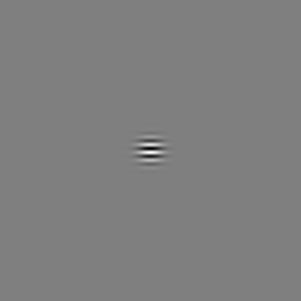
\includegraphics[width=\columnwidth/9]{ch4/figures/rGabor1_4.jpg}
 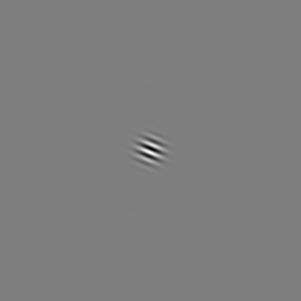
\includegraphics[width=\columnwidth/9]{ch4/figures/rGabor1_5.jpg}
 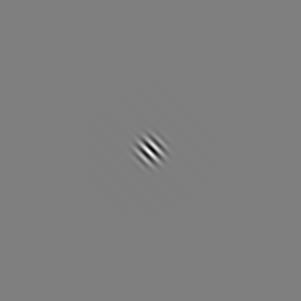
\includegraphics[width=\columnwidth/9]{ch4/figures/rGabor1_6.jpg}
 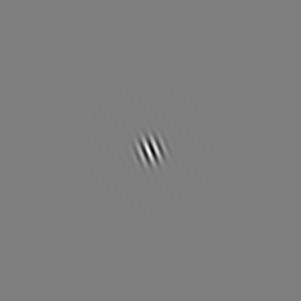
\includegraphics[width=\columnwidth/9]{ch4/figures/rGabor1_7.jpg}\\
 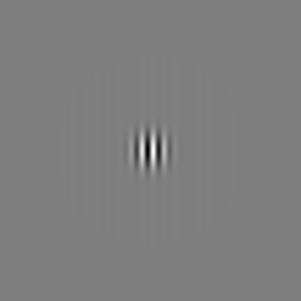
\includegraphics[width=\columnwidth/9]{ch4/figures/rGabor2_0.jpg}
 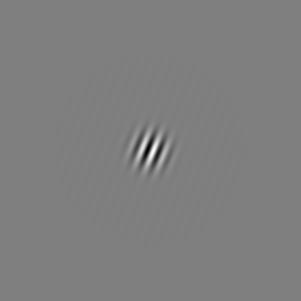
\includegraphics[width=\columnwidth/9]{ch4/figures/rGabor2_1.jpg}
 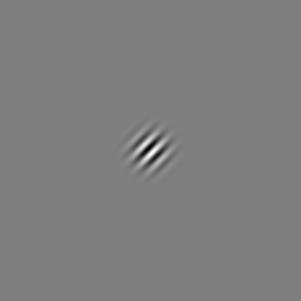
\includegraphics[width=\columnwidth/9]{ch4/figures/rGabor2_2.jpg}
 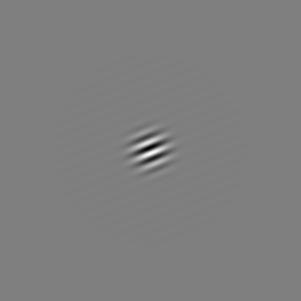
\includegraphics[width=\columnwidth/9]{ch4/figures/rGabor2_3.jpg}
 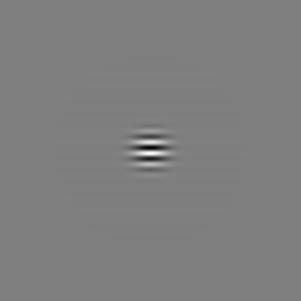
\includegraphics[width=\columnwidth/9]{ch4/figures/rGabor2_4.jpg}
 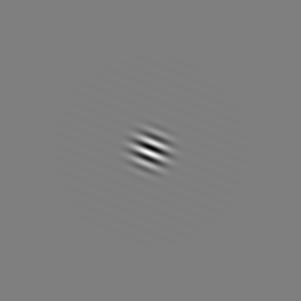
\includegraphics[width=\columnwidth/9]{ch4/figures/rGabor2_5.jpg}
 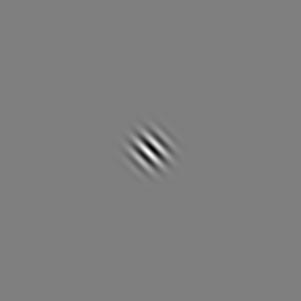
\includegraphics[width=\columnwidth/9]{ch4/figures/rGabor2_6.jpg}
 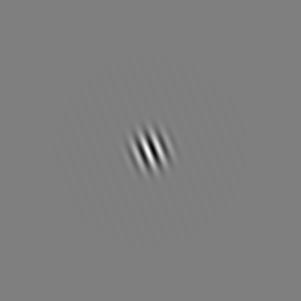
\includegraphics[width=\columnwidth/9]{ch4/figures/rGabor2_7.jpg}\\
 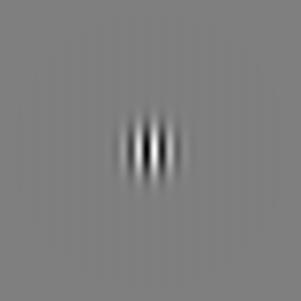
\includegraphics[width=\columnwidth/9]{ch4/figures/rGabor3_0.jpg}
 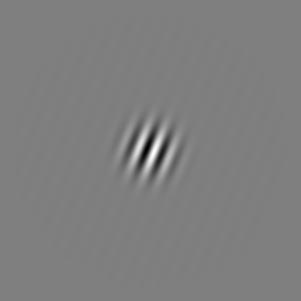
\includegraphics[width=\columnwidth/9]{ch4/figures/rGabor3_1.jpg}
 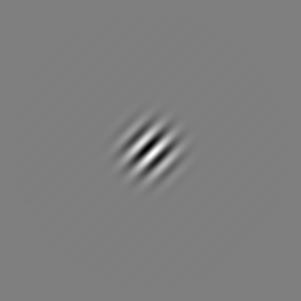
\includegraphics[width=\columnwidth/9]{ch4/figures/rGabor3_2.jpg}
 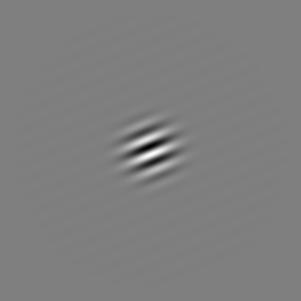
\includegraphics[width=\columnwidth/9]{ch4/figures/rGabor3_3.jpg}
 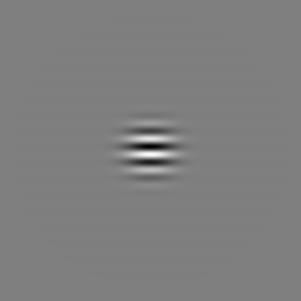
\includegraphics[width=\columnwidth/9]{ch4/figures/rGabor3_4.jpg}
 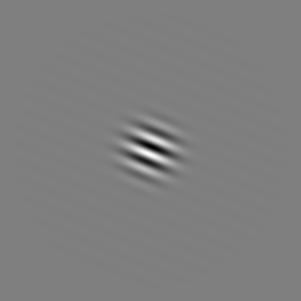
\includegraphics[width=\columnwidth/9]{ch4/figures/rGabor3_5.jpg}
 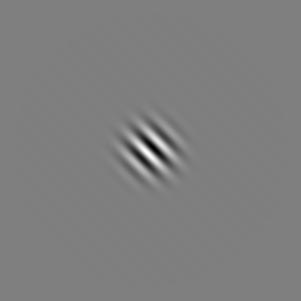
\includegraphics[width=\columnwidth/9]{ch4/figures/rGabor3_6.jpg}
 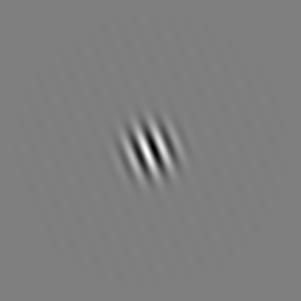
\includegraphics[width=\columnwidth/9]{ch4/figures/rGabor3_7.jpg}\\
 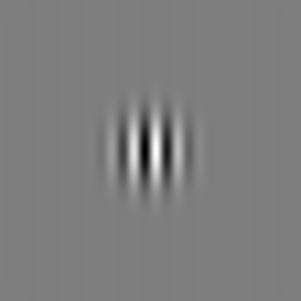
\includegraphics[width=\columnwidth/9]{ch4/figures/rGabor4_0.jpg}
 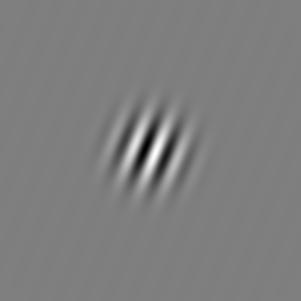
\includegraphics[width=\columnwidth/9]{ch4/figures/rGabor4_1.jpg}
 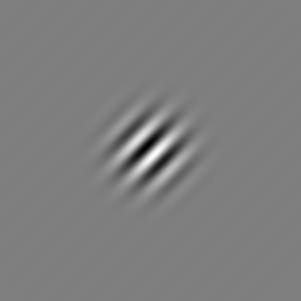
\includegraphics[width=\columnwidth/9]{ch4/figures/rGabor4_2.jpg}
 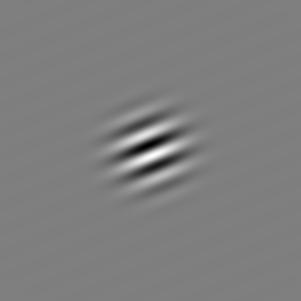
\includegraphics[width=\columnwidth/9]{ch4/figures/rGabor4_3.jpg}
 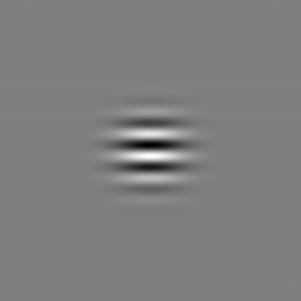
\includegraphics[width=\columnwidth/9]{ch4/figures/rGabor4_4.jpg}
 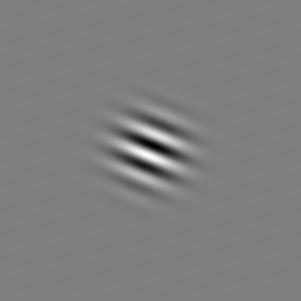
\includegraphics[width=\columnwidth/9]{ch4/figures/rGabor4_5.jpg}
 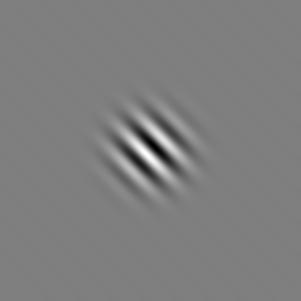
\includegraphics[width=\columnwidth/9]{ch4/figures/rGabor4_6.jpg}
 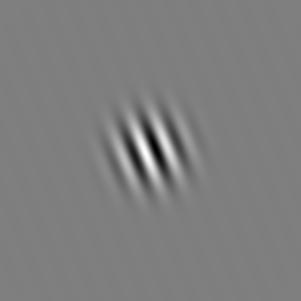
\includegraphics[width=\columnwidth/9]{ch4/figures/rGabor4_7.jpg}\\
\caption{The real part of the $5\times8$ Gabor wavelets.}
\label{fig:realgabor}
\end{center}
\end{figure} 
\begin{figure}[ht]
 \begin{center}
 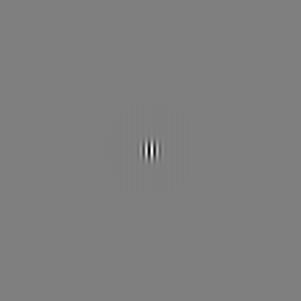
\includegraphics[width=\columnwidth/9]{ch4/figures/iGabor0_0.jpg}
 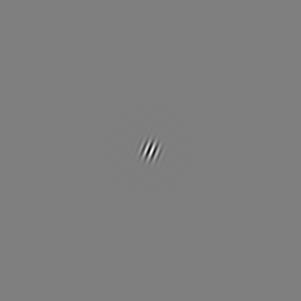
\includegraphics[width=\columnwidth/9]{ch4/figures/iGabor0_1.jpg}
 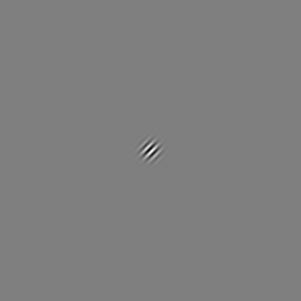
\includegraphics[width=\columnwidth/9]{ch4/figures/iGabor0_2.jpg}
 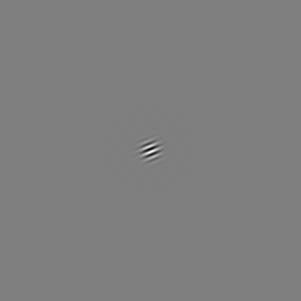
\includegraphics[width=\columnwidth/9]{ch4/figures/iGabor0_3.jpg}
 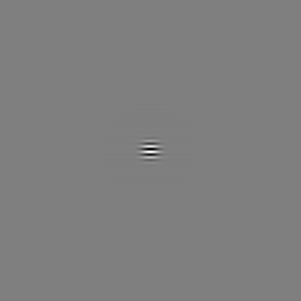
\includegraphics[width=\columnwidth/9]{ch4/figures/iGabor0_4.jpg}
 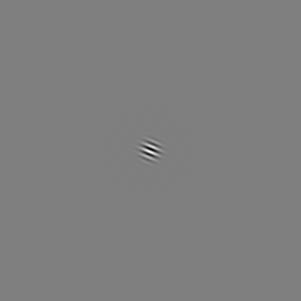
\includegraphics[width=\columnwidth/9]{ch4/figures/iGabor0_5.jpg}
 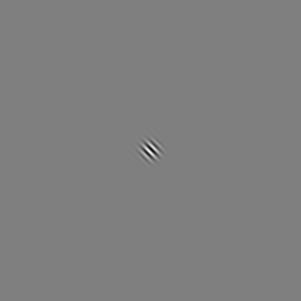
\includegraphics[width=\columnwidth/9]{ch4/figures/iGabor0_6.jpg}
 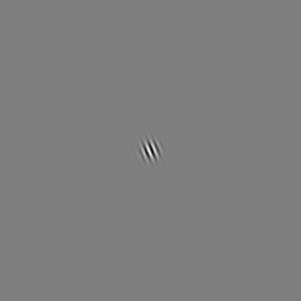
\includegraphics[width=\columnwidth/9]{ch4/figures/iGabor0_7.jpg}\\
 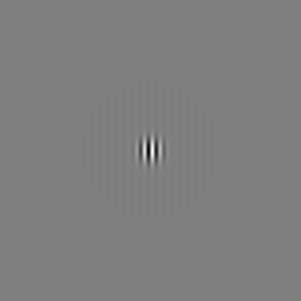
\includegraphics[width=\columnwidth/9]{ch4/figures/iGabor1_0.jpg}
 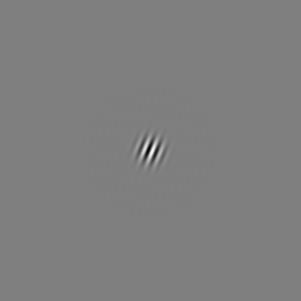
\includegraphics[width=\columnwidth/9]{ch4/figures/iGabor1_1.jpg}
 \includegraphics[width=\columnwidth/9]{ch4/figures/iGabor1_2.jpg}
 \includegraphics[width=\columnwidth/9]{ch4/figures/iGabor1_3.jpg}
 \includegraphics[width=\columnwidth/9]{ch4/figures/iGabor1_4.jpg}
 \includegraphics[width=\columnwidth/9]{ch4/figures/iGabor1_5.jpg}
 \includegraphics[width=\columnwidth/9]{ch4/figures/iGabor1_6.jpg}
 \includegraphics[width=\columnwidth/9]{ch4/figures/iGabor1_7.jpg}\\
 \includegraphics[width=\columnwidth/9]{ch4/figures/iGabor2_0.jpg}
 \includegraphics[width=\columnwidth/9]{ch4/figures/iGabor2_1.jpg}
 \includegraphics[width=\columnwidth/9]{ch4/figures/iGabor2_2.jpg}
 \includegraphics[width=\columnwidth/9]{ch4/figures/iGabor2_3.jpg}
 \includegraphics[width=\columnwidth/9]{ch4/figures/iGabor2_4.jpg}
 \includegraphics[width=\columnwidth/9]{ch4/figures/iGabor2_5.jpg}
 \includegraphics[width=\columnwidth/9]{ch4/figures/iGabor2_6.jpg}
 \includegraphics[width=\columnwidth/9]{ch4/figures/iGabor2_7.jpg}\\
 \includegraphics[width=\columnwidth/9]{ch4/figures/iGabor3_0.jpg}
 \includegraphics[width=\columnwidth/9]{ch4/figures/iGabor3_1.jpg}
 \includegraphics[width=\columnwidth/9]{ch4/figures/iGabor3_2.jpg}
 \includegraphics[width=\columnwidth/9]{ch4/figures/iGabor3_3.jpg}
 \includegraphics[width=\columnwidth/9]{ch4/figures/iGabor3_4.jpg}
 \includegraphics[width=\columnwidth/9]{ch4/figures/iGabor3_5.jpg}
 \includegraphics[width=\columnwidth/9]{ch4/figures/iGabor3_6.jpg}
 \includegraphics[width=\columnwidth/9]{ch4/figures/iGabor3_7.jpg}\\
 \includegraphics[width=\columnwidth/9]{ch4/figures/iGabor4_0.jpg}
 \includegraphics[width=\columnwidth/9]{ch4/figures/iGabor4_1.jpg}
 \includegraphics[width=\columnwidth/9]{ch4/figures/iGabor4_2.jpg}
 \includegraphics[width=\columnwidth/9]{ch4/figures/iGabor4_3.jpg}
 \includegraphics[width=\columnwidth/9]{ch4/figures/iGabor4_4.jpg}
 \includegraphics[width=\columnwidth/9]{ch4/figures/iGabor4_5.jpg}
 \includegraphics[width=\columnwidth/9]{ch4/figures/iGabor4_6.jpg}
 \includegraphics[width=\columnwidth/9]{ch4/figures/iGabor4_7.jpg}\\
\caption{The imaginary part of the $5\times8$ Gabor wavelets.}
\label{fig:imaggabor}
\end{center}
\end{figure} 
These Gabor wavelets share 5 scales and 8 orientations. The orientations from left to right are $0,\frac{\pi}{8},\frac{\pi}{4},\frac{3\pi}{8},\frac{\pi}{2},\frac{5\pi}{8},\frac{3\pi}{4},$ and $\frac{7\pi}{8}$. The scales from top to bottom are $-1$, $0$, $1$, $2$, $3$.

\subsection{Gabor Wavelet Transform}
\label{sec:gaborwavelettransform}
In computer vision, \textit{features} stand as a piece of ``interesting'' information which is relevant for solving a specific vision application. In appearance based approaches, features refer to the result after a general neighbourhood operation applied on an image. The result contains local or global information which contributes to resolving a specific vision problem. An image can be represented by a group of features. A computer vision system works on these features rather than image pixels directly.
Extraction of features is defined in terms of local neighbourhood operations. In this thesis, Gabor wavelet transform is the process to extract features which are relevant to face recognition. Since the selective schemes are available with a range of frequencies and orientation intervals, Gabor wavelets are ideal for face feature representation.

This section illustrates the Gabor wavelet transform by convolution. First of all, the concept of convolution is given. Secondly, the 2-D discrete convolution is presented. Thirdly, the size of mask for convolution is determined. Finally, the magnitude response is used as extracted features.
\subsubsection{Convolution}
The Gabor wavelet transform is the course of two-dimensional convolution of an image with a family of Gabor wavelet kernels defined by \mbox{Equation} \ref{eq:kernel}. Two-dimensional (2-D) convolution \cite{Sonka1998} is a specific type of local neighbourhood operation which belongs to the linear approach in image analysis. The 2-D convolution $g$ of two-dimensional functions $f$ and $h$ is denoted by $f*h$. The function of 2-D convolution is expressed as
\newcommand{\ud}{\mathrm{d}}
{\setlength\arraycolsep{2pt}
\begin{eqnarray}\label{eq:conv2}
 g(x, y) = \int_{-\infty}^{\infty}\int_{-\infty}^{\infty}f(a,b)h(x-a,y-b) \, \ud a \, \ud b \nonumber\\
= \int_{-\infty}^{\infty}\int_{-\infty}^{\infty}f(x-a,y-b)h(a,b) \, \ud a \, \ud b \nonumber\\
= (f*h)(x,y) = (h*f)(x,y) ��\end{eqnarray}
} 
where the operator $*$ symbolise the convolution operator. The 2-D convolution is an integral of the functions $f$ and $h$. The convolution means a linear filtering process using the filter $h$ on the image $f$.  The linear filtering is often used in local image pre-processing.

\subsubsection{2-D discrete convolution}
In the 2-D discrete image domain, the linear filtering calculates the image pixel $g(x,y)$ as a linear combination of the pixel value in a local neighbourhood of the pixel $f(a,b)$. The 2-D discrete convolution is described as
\begin{equation}
 %g(x,y)=\sum^{\infty}_{a=-\infty}\sum^{\infty}_{b=-\infty}f(a,b)h(x-a,y-b)
g(x,y)=\sum_{a}\sum_{b}f(a,b)h(x-a,y-b)
\end{equation}
where $f(a,b)$ is the 2-D discrete input image and $h(x,y)$ is the so-called \textbf{convolution mask} or convolution kernel. The convolution mask is often used with an odd number of pixels in rows and columns, such as $3\times3$, $5\times5$ and so on. An example \cite{Davies1990} of a $3\times3$ convolution mask is
\begin{displaymath}
 \left[  \begin{array}{ccc}
          \mathrm{h}_{4} &\mathrm{h}_{3} & \mathrm{h}_{2} \\
	  \mathrm{h}_{5} & \mathrm{h}_{0} & \mathrm{h}_{1} \\
	  \mathrm{h}_{6} & \mathrm{h}_{7} & \mathrm{h}_{8} 
         \end{array}
\right ]
\end{displaymath}
where $\mathrm{h}_{n}$ is the coefficient of the convolution mask. The 2-D convolution result is the linear neighbourhood operation weighted by the corresponding coefficients in the mask $h$. In practice, fast convolution is used to increase the speed of the convolution. A fast convolution algorithm takes the fast Fourier transform (FFT) of the input image and the convolution mask, multiplies them together, and then performs the inverse fast Fourier transform (IFFT). In this thesis, the 2-D discrete convolution function is provided by OpenCV \cite{Landre2003} in implementation.
\subsubsection{The Size of Mask}
In 2-D discrete convolution, the size of a Gabor filtering convolution mask is an important issue. It should be large enough to show the nature of Gabor wavelets. However, it should not be too large, otherwise computation cost will be increased. For instance, in \mbox{Figure} \ref{fig:realgabor}, the size of the Gabor convolution masks is $301\times301$, and the Gabor wavelets with the lowest frequency are shown on the top row. The span of these Gabor masks only possess a small part at the centre of the mask, and the rest of the area conveys no information. The size of a Gabor mask should be large enough to cover the shape of Gabor wavelet. The size of Gabor wavelet is determined by the spatial extent of the Gaussian envelope, which is then determined by the spatial frequency $\nu$ and the deviation of Gaussian function $\sigma$ in \mbox{Equation} \ref{eq:kernel}. According to Dunn \textit{et al.} \cite{Dunn1995}, the Gabor filter is truncated to six times the span of the Gaussian function. The span of Gaussian function is $\frac{\sigma}{\|k_{\nu}\|}$ and $k_{\nu}=\frac{k_{max}}{f^{\nu}}$, so that the Gabor mask is truncated to a width $W$
 \begin{equation}
  W  = \frac{6\sigma}{\|k_{\nu}\|}+1 = 6 f^{\nu}\frac{\sigma}{k_{max}}+1
 \end{equation}
Taking $k_{max}=\frac{\pi}{2}$, the factor $f = \sqrt{2}$ and the standard deviation of the Gaussian $\sigma=2\pi$, the width is 
\begin{equation}
 W = 24\cdot2^{\frac{\nu}{2}}+1
\end{equation}
For five different spatial frequencies $\nu\in\{-1,\ldots,3\}$, the corresponding size of Gabor filtering masks are $19\times19$, $25\times25$, $35\times35$, $49\times49$ and $69\times69$. \mbox{Figure} \ref{fig:fivemasks} with the $\frac{3\pi}{8}$ orientation, the corresponding real masks with the different spatial frequencies.
\begin{figure}[ht]
\begin{center}
\includegraphics[scale=1.0]{ch4/figures/real-1.jpg}
\includegraphics[scale=1.0]{ch4/figures/real0.jpg}
\includegraphics[scale=1.0]{ch4/figures/real1.jpg}
\includegraphics[scale=1.0]{ch4/figures/real2.jpg}
\includegraphics[scale=1.0]{ch4/figures/real3.jpg}\\
\caption{When orientation $\mu = 3$, \textit{i.e.}, $\frac{3\pi}{8}$,the corresponding Gabor filtering convolution masks with the five different spatial frequencies $\nu\in\{-1,\ldots,3\}$.} 
\label{fig:fivemasks}
\end{center}
\end{figure} 

\subsubsection{Magnitude Response} 
To get the Gabor wavelet transform of an image, the 40 Gabor wavelets are convolved with the image. Let $I(z)$, where $z=(x,y)$ defines the position in the image, the convolution of an image $I$ and a Gabor kernel $\psi_{\mu,\nu}$ is defined as
\begin{equation}\label{eq:conv}
 O_{\mu,\nu}(z)=I(z)\ast\psi_{\mu,\nu}(z)
\end{equation}
where $*$ denotes the convolution operator, and $O_{\mu,\nu}$ is the convolution result corresponding to the Gabor kernel at the orientation $\mu$ and the spatial frequency $\nu$.\footnote{In some cases, the spatial frequency $\nu$ is also called scale.} Since Gabor wavelets are of the complex form, the convolution results contain the real response and imaginary response as follow
\begin{displaymath}
 O_{\mu,\nu}(z) = \Re\{O_{\mu,\nu}(z)\} +i\,\Im\{O_{\mu,\nu}(z)\}
\end{displaymath}
where $\Re$ represents the real response and $\Im$ represents the imaginary response. The real response of Gabor filtering is an image $I(z)$ convolved with the real unit of Gabor kernel described as (\ref{eq:real}). The real response of Gabor filtering is 
\begin{equation}
 \Re\{O_{\mu,\nu}(z)\} = I(z) *  \Re\{\psi_{\mu,\nu}\}
\end{equation}
The imaginary response is the image convolved with the imaginary part described as \mbox{Equation} \ref{eq:imag}. It is expressed as
\begin{equation}
 \Im\{O_{\mu,\nu}(z)\} = I(z) *  \Im\{\psi_{\mu,\nu}\}
\end{equation}
Given a face image shown in \mbox{Figure} \ref{fig:afaceimage} in the \textbf{FERET} database \cite{Phillips2000}, 
\begin{figure}[t]
 \begin{center}
   \includegraphics[scale=0.75]{ch4/figures/FERET.jpg}
   \caption{A face image selected from the \textbf{FERET} database.}
   \label{fig:afaceimage}
 \end{center}
\end{figure} 
the 40 Gabor real responses and imaginary responses are displayed in \mbox{Figure} \ref{fig:realresponses} and \mbox{Figure} \ref{fig:imagresponses} respectively.
\begin{figure}[ht]
 \begin{center}
  \includegraphics[width=\columnwidth/9]{ch4/figures/real_-1_0.jpg}
  \includegraphics[width=\columnwidth/9]{ch4/figures/real_-1_1.jpg}
  \includegraphics[width=\columnwidth/9]{ch4/figures/real_-1_2.jpg}
  \includegraphics[width=\columnwidth/9]{ch4/figures/real_-1_3.jpg}
  \includegraphics[width=\columnwidth/9]{ch4/figures/real_-1_4.jpg}
  \includegraphics[width=\columnwidth/9]{ch4/figures/real_-1_5.jpg}
  \includegraphics[width=\columnwidth/9]{ch4/figures/real_-1_6.jpg}
  \includegraphics[width=\columnwidth/9]{ch4/figures/real_-1_7.jpg}\\
  \includegraphics[width=\columnwidth/9]{ch4/figures/real_0_0.jpg}
  \includegraphics[width=\columnwidth/9]{ch4/figures/real_0_1.jpg}
  \includegraphics[width=\columnwidth/9]{ch4/figures/real_0_2.jpg}
  \includegraphics[width=\columnwidth/9]{ch4/figures/real_0_3.jpg}
  \includegraphics[width=\columnwidth/9]{ch4/figures/real_0_4.jpg}
  \includegraphics[width=\columnwidth/9]{ch4/figures/real_0_5.jpg}
  \includegraphics[width=\columnwidth/9]{ch4/figures/real_0_6.jpg}
  \includegraphics[width=\columnwidth/9]{ch4/figures/real_0_7.jpg}\\
  \includegraphics[width=\columnwidth/9]{ch4/figures/real_1_0.jpg}
  \includegraphics[width=\columnwidth/9]{ch4/figures/real_1_1.jpg}
  \includegraphics[width=\columnwidth/9]{ch4/figures/real_1_2.jpg}
  \includegraphics[width=\columnwidth/9]{ch4/figures/real_1_3.jpg}
  \includegraphics[width=\columnwidth/9]{ch4/figures/real_1_4.jpg}
  \includegraphics[width=\columnwidth/9]{ch4/figures/real_1_5.jpg}
  \includegraphics[width=\columnwidth/9]{ch4/figures/real_1_6.jpg}
  \includegraphics[width=\columnwidth/9]{ch4/figures/real_1_7.jpg}\\
  \includegraphics[width=\columnwidth/9]{ch4/figures/real_2_0.jpg}
  \includegraphics[width=\columnwidth/9]{ch4/figures/real_2_1.jpg}
  \includegraphics[width=\columnwidth/9]{ch4/figures/real_2_2.jpg}
  \includegraphics[width=\columnwidth/9]{ch4/figures/real_2_3.jpg}
  \includegraphics[width=\columnwidth/9]{ch4/figures/real_2_4.jpg}
  \includegraphics[width=\columnwidth/9]{ch4/figures/real_2_5.jpg}
  \includegraphics[width=\columnwidth/9]{ch4/figures/real_2_6.jpg}
  \includegraphics[width=\columnwidth/9]{ch4/figures/real_2_7.jpg}\\
  \includegraphics[width=\columnwidth/9]{ch4/figures/real_3_0.jpg}
  \includegraphics[width=\columnwidth/9]{ch4/figures/real_3_1.jpg}
  \includegraphics[width=\columnwidth/9]{ch4/figures/real_3_2.jpg}
  \includegraphics[width=\columnwidth/9]{ch4/figures/real_3_3.jpg}
  \includegraphics[width=\columnwidth/9]{ch4/figures/real_3_4.jpg}
  \includegraphics[width=\columnwidth/9]{ch4/figures/real_3_5.jpg}
  \includegraphics[width=\columnwidth/9]{ch4/figures/real_3_6.jpg}
  \includegraphics[width=\columnwidth/9]{ch4/figures/real_3_7.jpg}\\
\caption{The 40 real response images.}
\label{fig:realresponses}
 \end{center}
\end{figure} 
\begin{figure}
 \begin{center}
  \includegraphics[width=\columnwidth/9]{ch4/figures/imag_-1_0.jpg}
  \includegraphics[width=\columnwidth/9]{ch4/figures/imag_-1_1.jpg}
  \includegraphics[width=\columnwidth/9]{ch4/figures/imag_-1_2.jpg}
  \includegraphics[width=\columnwidth/9]{ch4/figures/imag_-1_3.jpg}
  \includegraphics[width=\columnwidth/9]{ch4/figures/imag_-1_4.jpg}
  \includegraphics[width=\columnwidth/9]{ch4/figures/imag_-1_5.jpg}
  \includegraphics[width=\columnwidth/9]{ch4/figures/imag_-1_6.jpg}
  \includegraphics[width=\columnwidth/9]{ch4/figures/imag_-1_7.jpg}\\
  \includegraphics[width=\columnwidth/9]{ch4/figures/imag_0_0.jpg}
  \includegraphics[width=\columnwidth/9]{ch4/figures/imag_0_1.jpg}
  \includegraphics[width=\columnwidth/9]{ch4/figures/imag_0_2.jpg}
  \includegraphics[width=\columnwidth/9]{ch4/figures/imag_0_3.jpg}
  \includegraphics[width=\columnwidth/9]{ch4/figures/imag_0_4.jpg}
  \includegraphics[width=\columnwidth/9]{ch4/figures/imag_0_5.jpg}
  \includegraphics[width=\columnwidth/9]{ch4/figures/imag_0_6.jpg}
  \includegraphics[width=\columnwidth/9]{ch4/figures/imag_0_7.jpg}\\
  \includegraphics[width=\columnwidth/9]{ch4/figures/imag_1_0.jpg}
  \includegraphics[width=\columnwidth/9]{ch4/figures/imag_1_1.jpg}
  \includegraphics[width=\columnwidth/9]{ch4/figures/imag_1_2.jpg}
  \includegraphics[width=\columnwidth/9]{ch4/figures/imag_1_3.jpg}
  \includegraphics[width=\columnwidth/9]{ch4/figures/imag_1_4.jpg}
  \includegraphics[width=\columnwidth/9]{ch4/figures/imag_1_5.jpg}
  \includegraphics[width=\columnwidth/9]{ch4/figures/imag_1_6.jpg}
  \includegraphics[width=\columnwidth/9]{ch4/figures/imag_1_7.jpg}\\
  \includegraphics[width=\columnwidth/9]{ch4/figures/imag_2_0.jpg}
  \includegraphics[width=\columnwidth/9]{ch4/figures/imag_2_1.jpg}
  \includegraphics[width=\columnwidth/9]{ch4/figures/imag_2_2.jpg}
  \includegraphics[width=\columnwidth/9]{ch4/figures/imag_2_3.jpg}
  \includegraphics[width=\columnwidth/9]{ch4/figures/imag_2_4.jpg}
  \includegraphics[width=\columnwidth/9]{ch4/figures/imag_2_5.jpg}
  \includegraphics[width=\columnwidth/9]{ch4/figures/imag_2_6.jpg}
  \includegraphics[width=\columnwidth/9]{ch4/figures/imag_2_7.jpg}\\
  \includegraphics[width=\columnwidth/9]{ch4/figures/imag_3_0.jpg}
  \includegraphics[width=\columnwidth/9]{ch4/figures/imag_3_1.jpg}
  \includegraphics[width=\columnwidth/9]{ch4/figures/imag_3_2.jpg}
  \includegraphics[width=\columnwidth/9]{ch4/figures/imag_3_3.jpg}
  \includegraphics[width=\columnwidth/9]{ch4/figures/imag_3_4.jpg}
  \includegraphics[width=\columnwidth/9]{ch4/figures/imag_3_5.jpg}
  \includegraphics[width=\columnwidth/9]{ch4/figures/imag_3_6.jpg}
  \includegraphics[width=\columnwidth/9]{ch4/figures/imag_3_7.jpg}\\
\caption{The 40 imaginary responses}
\label{fig:imagresponses}
 \end{center}
\end{figure} 
From \mbox{Figures} \ref{fig:realresponses} and \ref{fig:imagresponses}, it is hard to see a human face rather than the stripes across the images.

Texture detection can be operated based on the magnitude of the output of the Gabor filtering \cite{Bovik1990}. The magnitude response of Gabor filtering is widely used in texture detection. Since the human face contains various textures, the magnitude response of Gabor filtering will enhance the recognition of a face. It is the square root of the sum of the squared real response and imaginary response, such as
\begin{equation}
 \|O_{\mu,\nu}(z)\| = \sqrt{\Re^2\{O_{\mu,\nu}(z)\} + \Im^2\{O_{\mu,\nu}(z)\}}
\end{equation}
It can be seen that the magnitude response is modulus. These 40 Gabor magnitude responses are shown in \mbox{Figure} \ref{fig:magresponses} relating to the image shown in \mbox{Figure} \ref{fig:afaceimage}.
\begin{figure}[ht]
\begin{center}
 \includegraphics[width=\columnwidth/9]{ch4/figures/mag_-1_0.jpg}
 \includegraphics[width=\columnwidth/9]{ch4/figures/mag_-1_1.jpg}
 \includegraphics[width=\columnwidth/9]{ch4/figures/mag_-1_2.jpg}
 \includegraphics[width=\columnwidth/9]{ch4/figures/mag_-1_3.jpg}
 \includegraphics[width=\columnwidth/9]{ch4/figures/mag_-1_4.jpg}
 \includegraphics[width=\columnwidth/9]{ch4/figures/mag_-1_5.jpg}
 \includegraphics[width=\columnwidth/9]{ch4/figures/mag_-1_6.jpg}
 \includegraphics[width=\columnwidth/9]{ch4/figures/mag_-1_7.jpg}\\
 \includegraphics[width=\columnwidth/9]{ch4/figures/mag_0_0.jpg}
 \includegraphics[width=\columnwidth/9]{ch4/figures/mag_0_1.jpg}
 \includegraphics[width=\columnwidth/9]{ch4/figures/mag_0_2.jpg}
 \includegraphics[width=\columnwidth/9]{ch4/figures/mag_0_3.jpg}
 \includegraphics[width=\columnwidth/9]{ch4/figures/mag_0_4.jpg}
 \includegraphics[width=\columnwidth/9]{ch4/figures/mag_0_5.jpg}
 \includegraphics[width=\columnwidth/9]{ch4/figures/mag_0_6.jpg}
 \includegraphics[width=\columnwidth/9]{ch4/figures/mag_0_7.jpg}\\
 \includegraphics[width=\columnwidth/9]{ch4/figures/mag_1_0.jpg}
 \includegraphics[width=\columnwidth/9]{ch4/figures/mag_1_1.jpg}
 \includegraphics[width=\columnwidth/9]{ch4/figures/mag_1_2.jpg}
 \includegraphics[width=\columnwidth/9]{ch4/figures/mag_1_3.jpg}
 \includegraphics[width=\columnwidth/9]{ch4/figures/mag_1_4.jpg}
 \includegraphics[width=\columnwidth/9]{ch4/figures/mag_1_5.jpg}
 \includegraphics[width=\columnwidth/9]{ch4/figures/mag_1_6.jpg}
 \includegraphics[width=\columnwidth/9]{ch4/figures/mag_1_7.jpg}\\
 \includegraphics[width=\columnwidth/9]{ch4/figures/mag_2_0.jpg}
 \includegraphics[width=\columnwidth/9]{ch4/figures/mag_2_1.jpg}
 \includegraphics[width=\columnwidth/9]{ch4/figures/mag_2_2.jpg}
 \includegraphics[width=\columnwidth/9]{ch4/figures/mag_2_3.jpg}
 \includegraphics[width=\columnwidth/9]{ch4/figures/mag_2_4.jpg}
 \includegraphics[width=\columnwidth/9]{ch4/figures/mag_2_5.jpg}
 \includegraphics[width=\columnwidth/9]{ch4/figures/mag_2_6.jpg}
 \includegraphics[width=\columnwidth/9]{ch4/figures/mag_2_7.jpg}\\
 \includegraphics[width=\columnwidth/9]{ch4/figures/mag_3_0.jpg}
 \includegraphics[width=\columnwidth/9]{ch4/figures/mag_3_1.jpg}
 \includegraphics[width=\columnwidth/9]{ch4/figures/mag_3_2.jpg}
 \includegraphics[width=\columnwidth/9]{ch4/figures/mag_3_3.jpg}
 \includegraphics[width=\columnwidth/9]{ch4/figures/mag_3_4.jpg}
 \includegraphics[width=\columnwidth/9]{ch4/figures/mag_3_5.jpg}
 \includegraphics[width=\columnwidth/9]{ch4/figures/mag_3_6.jpg}
 \includegraphics[width=\columnwidth/9]{ch4/figures/mag_3_7.jpg}\\
 \caption{The 40 magnitude responses}
\label{fig:magresponses}
\end{center}
\end{figure} 
The magnitude responses demonstrate local variance within low spatial-frequency and global variance within high spatial-frequency. In the top rows, more precise dissimilarity across the face are shown, while in the bottom rows, more high-level scale dissimilarity across the face are shown. In this thesis, the magnitude response of Gabor filtering is adopted to extract Gabor Wavelet Features. 


\subsection{Gabor Wavelet Feature}
\label{sec:gaborwaveletfeature}
As stated before, a Gabor wavelet feature $j$ is configured by three key parameters: the position $z = (x,y)$, the orientation $\nu$, and the spatial frequency $\mu$. The value of a Gabor wavelet feature is the corresponding magnitude response of a Gabor wavelet transform
\begin{equation}\label{eq:gaborfeature}
 j(z,\nu,\mu) =  \|O_{\mu,\nu}(z)\|
\end{equation}
Gabor wavelet features vary in orientation, frequency and position. There are eight different orientations from $0$ to $\frac{7\pi}{8}$ with the interval $\frac{\pi}{8}$, and five different scales from $-1$ to $3$.  These 40 Gabor wavelets are applied on every position on a face image, so that the total number of Gabor wavelet features is determined by the number of orientations, the number of scales, and the resolution (size) of the image  applied. For example, for an image with $64\times 64$ pixels, the total number of Gabor wavelet features is $64\times 64\times 5\times 8=163,840$. If the number of Gabor wavelets is fixed, the only factor which changes the total number of features is the size of the image.


\section{AdaBoost}
\label{sec:faceveri:adaboost}
AdaBoost, standing for Adaptive Boosting, is a machine learning algorithm, formulated by Freund and Schapire \cite{Freund1995,Freund1999,Schapire1999}. AdaBoost can be used in conjunction with many other learning algorithms to improve their performance and learning accuracy.

This section gives a description of AdaBoost. In \mbox{Section} \ref{sec:adaboostintro}, a brief introduction of AdaBoost with a horse-racing analogy is given. \mbox{Section} \ref{sec:adaboostaglortihm} presents the AdaBoost algorithm, and \mbox{Section} \ref{sec:adaboostconstruction} describes how a ``strong'' ensemble classifier is constructed by a number of ``weak'' learners. Finally, an experiment of AdaBoost training and classification is given in \mbox{Section} \ref{sec:irisexp} in the Iris dataset.

\subsection{Introduction to AdaBoost}
\label{sec:adaboostintro}
Boosting is a general method which is used to ``boost'' the accuracy of any given learning algorithm. Boosting is originated in a theoretical framework for machine learning called ``PAC'' (Probably Approximately Correct) learning model \cite{Valiant1984}. After the PAC releasing,  there is a discussion whether a ``weak'' learning algorithm performing just slightly better than random guessing can be boosted into an arbitrarily accurate ``strong'' learning algorithm. Kearns and Valiant \cite{Kearns1994} are first to respond to the discussion with the positive answer. In 1989, Schapire proposed the first provable polynomial-time boosting algorithm \cite{Schapire1990}. Boosting is firstly applied to real-world application for an Optical Character Recognition (OCR) task, relying on neural networks as base learners in \cite{Drucker1993}. Although  Freund and Schapire \cite{Freund1995,Freund1999,Schapire1999} claims that AdaBoost often tends not to overfit when running for a large number of iterations, other simulations \cite{Grove1998} on data sets with higher noise content could clearly show overfitting side-effects. Due to the accuracy of Boosting, the algorithm has been extended for regression \cite{Friedman1998}, multi-class classification \cite{Zhu2006}, and unsupervised learning \cite{Ratsch2002}. Recently, Boosting has been successfully implemented in various applications. OCR \cite{Drucker1993} is implemented, which used boosted classifier of neural network. In human face detection, AdaBoost was used to train a ``strong'' classifier to detect faces in an image \cite{Viola2001,Viola2004}.

\paragraph{Horse-racing analogy}
An analogy \cite{Freund1995,Freund1999,Schapire1999} between the AdaBoost algorithm and horse-racing gambling is drawn for a better understanding on AdaBoost. A horse-racing gambler, whose purpose is to maximise his winning, wants to create a computer program helping his betting. The program would accurately predict the winner of a horse race. To create such a program, he consults a successful horse-racing gambling expert for the optimal rule to bet. However, the expert fails to answer, because the expert can not articulate a grand set of rules for choosing a winning horse. On the other hand, when the gambler provides the specific data of races to the expert, the expert can easily come up with a ``rule of thumb'' for the set of races. The possible ``rule of thumb'' is like ``betting on the horse that has recently won the most races'' or ``betting on the horse with the most favoured odds''. The rule of thumb is very rough and moderately inaccurate, but the rule is quite reasonable. The rule can be easily concluded from the specific data rather than from a random guess. If the gambler keeps on asking the expert on different collections of races, the expert would draw many rules of thumb. To get the maximum advantage from these rules of thumb, two problems must be resolved.
\begin{itemize}
 \item How could the gambler choose the collections of races which are given to the expert for extracting the most useful rules of thumb?
 \item  When many rules of thumb are extracted, how are these rules combined into one single accurate rule?
\end{itemize}

\subsection{AdaBoost algorithm}
\label{sec:adaboostaglortihm}
AdaBoost is an efficient method of producing a highly accurate predication rule by combining a set of rough and moderately inaccurate rules of thumb. In general, the so-called ``rule of thumb'' is simply designed rules which give low accuracy over long-term observation. For computer vision and pattern recognition, the word ``rule'' is replaced by the word ``classifier'', ``learner'', ``hypothesis'', etc. In this thesis, the term ``learner'' is used.  For the term ``rule of thumb'', it is called \textit{weak learner}. AdaBoost refers to a method of combining a set of ``weak'' learner into a ``strong'' classifier which gives a high accuracy for prediction. In order to design the ``strong'' classifier, two issues need to be resolved
\begin{itemize}
 \item How is a set of ``weak'' learners organised into a ``strong'' classifier?
 \item How is a ``weak'' learner selected so that it contributes to a ``strong'' classifier?
\end{itemize}
AdaBoost resolves these two problems and gives the better performance of classification.

The AdaBoost algorithm is introduced to solve the difficulties of the earlier boosting algorithm. AdaBoost is an \textit{adaptive} boosting algorithm, because AdaBoost adapts to the error rates of individual ``weak'' classifier. Pseudocode for AdaBoost is given in \mbox{Table} \ref{tab:adaboost}. 
\begin{table}
\caption{The AdaBoost algorithm}

\begin{tabular}{p{\columnwidth}}
\hline
 \begin{algorithmic}[1]
\STATE Given the training set $(x_{1},y_{1}),\ldots,(x_{n},y_{n})$, where $x_{i}$ is the data of the $i$th example, and $y_{i} \in Y=\{0,1\}$.
\STATE Initialise the weights $\omega_{1,i}=\frac{1}{n}$ for each example $(x_{i},y_{i})$.
\FOR{$t=1,\ldots,T$}
	\STATE Train a weak learner $h_{t}$ using the weights $\omega_{t,i}$.
	\STATE Get the weak learner with error 
                       \begin{equation}\label{eq:error}
                        \varepsilon_{t} =\sum_{i=0}^{n}\omega_{t,i}\|h_{t}(x_{i})-y_{i}\|^2
                       \end{equation}
	\STATE Choose $\alpha_{t}=\frac{1}{2}\ln \left( \frac{1-\varepsilon_{t}}{\varepsilon_{t}} \right)$
	\STATE Update the weights 
		\begin{equation}\label{eq:update}
		 \omega_{t,i} = \omega_{t,i} \times
                 \left\{
		  \begin{array}{ll}
		                                            e^{-\alpha_{t}} & \textrm{if $h_{t}(x_{i})=y_{i}$} \\
						           e^{\alpha_{t}} & \textrm{if $h_{t}(x_{i}) \neq y_{i}$}
		  \end{array}
		\right.
		\end{equation}
	\STATE Normalise the weights 
		\begin{equation}\label{eq:normalisation}
		  \omega_{t+1,i} = \frac{\omega_{t,i}}{\sum_{i=1}^{n}\omega_{t,i}}
		\end{equation}
	where the normalisation can be expressed by a normalisation factor $Z_{t}$ so that all $ \omega_{t+1,i}$ will keep a probability distribution.
\ENDFOR
\STATE The final ``strong'' (ensemble) classifier:
	\begin{equation}
	 H(x)  = 
		\left\{
		 \begin{array}{ll}
		  1 & \sum_{t=1}^{T}\alpha_{t}h_{t}(x) \geq \frac{1}{2}\sum_{t=1}^{T}\alpha_{t}\\
			\\
		  0 & \textrm{otherwise}
		 \end{array}
		\right. 
	\end{equation}
\end{algorithmic}\\
\hline
\label{tab:adaboost}
\end{tabular}
\end{table} 

\paragraph{Training Data}There are $n$ examples in the training set $(x_{1},y_{1}),\ldots,(x_{n},y_{n})$. $x$ is the data of the example which can be integer or real, positive or negative. $y$ is the label of the example, and it is assumed that $y \in \{0,1\}$. In this chapter, only the two-class classification is discussed\footnote{\mbox{Chapter} \ref{ch:multi} gives the description of multi-class classification.}. AdaBoost maintains a collection of weights on each example. All the weights $\omega_{t}$ are kept as a probability distribution $D_{t}$.
\begin{equation}\label{eq:distribution}\nonumber
 D_{t}(i) = \omega_{t,i}
\end{equation}
At the beginning, the distribution $D_{t}$ is uniform such that all weights are equal to $1/n$. 

\paragraph{Weak Learner}
AdaBoost processes ``weak'' classifiers repeatedly in $t=1,\ldots,T$ iteration. In each iteration, a ``weak'' learner $h_{t}$ is trained by using the distribution $D_{t}$. To train a weak learner, there are many approaches, \textit{e.g.}, Naive Bayes \cite{Domingos1997}, Perceptron \cite{Rosenblatt1958}, Linear Discriminant Analysis (LDA) \cite{Martinez2001}, Neural network \cite{Riedmiller1993}, etc. When $h_{t}$ is trained, the calculation of the error $\varepsilon_{t}$ is shown in \mbox{Equation} \ref{eq:error}. When an example $(x_{i},y_{i})$ is misclassified by the weak learner $h_{t}$, \textit{i.e.}, $h_{t}(x_{i})\neq y_{i}$, the weight  $\omega_{t,i}$ is added in error $\varepsilon_{t}$. When an example is classified, the weight will not be counted in $\varepsilon_{t}$.
The smaller the $\varepsilon_t$ is, the stronger is the weak learner $h_t$. Normally, the error $\varepsilon_{t}$ is relative large, but does not exceed $0.5$. In practice, a weak learner is a learning algorithm that can use the weights $\omega_{t,i}$ on the training data.
%Recalling the horse-racing analogy, $x_{i}$ of the example $(x_{i},y_{i})$ corresponds to information revelant to horse races, \textit{e.g.}, the name of horse, the odds, the track record of horse, the weather of the racing day, the condition of race course, etc.  The label $y_{i}$ gives the result of each race, i.e. who is the winner. The weak learners are the rules of thumb given by the expert. 

\paragraph{Importance}Once a weak learner has been trained, AdaBoost will determine a parameter $\alpha_{t}$, which indicates how important the corresponding weak learner $h_{t}$ is  in the final classifier $H(x)$. When $\alpha_{t}$ is larger, the corresponding weak learner $h_{t}$ contributes more in $H(x)$. Note that $\alpha_{t} \geq 0$ if $\varepsilon_{t} \leq \frac{1}{2}$, such that $\alpha_{t}$ gets larger as $\varepsilon_{t}$ gets smaller.

\paragraph{Updating}The weight $\omega_{t,i}$ is updated using the rule shown in \mbox{Equation} \ref{eq:update}. The effect of the updating weight is to increase the weight of examples misclassified, and to decrease the weight of correctly classified examples. In this way, AdaBoost is modulated to focus on those examples which are ``hard'' to classify.

\paragraph{Normalisation}The updated weights are normalised by a normalisation operator $Z_{t}$. After updating the weights, all the weights may not constitute a probability distribution, \textit{i.e.}, the sum of all weights may not be equal to $1$. To forge the weights into a probability distribution, all the weights for the next iteration will be normalised according to \mbox{Equation} \ref{eq:normalisation}. $\omega_{t+1,i}$ is increased to the example $x_{i}$ over other examples, when $x_{i}$ is misclassified and other examples are classified correctly in the $t$th iteration. In general, the weights only increase or decrease in a relative manner.

\paragraph{Final classifier}
The final ``strong'' classifier $H(x)$ is a weighted majority vote of the $T$ weak learners where $\alpha_{t}$ is the weight assigned to $h_{t}$. The ``strong'' classifier is called \textbf{ensemble}, which refers to a collection of statistical classifiers. An ensemble classifier consists of a set of individually trained classifiers, i.e., weak learners, whose predictions are combined. Previous research \cite{Opitz1999} has shown that an ensemble classifier is often more accurate than any of the single classifier in the ensemble. Bagging \cite{Breiman1996} and Boosting \cite{Freund1996} are two relatively new but popular methods for producing ensemble classifiers. Bagging is a ``bootstrap'' \cite{Efron1993} ensemble method that creates individual classifiers for its ensemble by training each classifier on a random redistribution of the training set. However, Boosting is focusing on producing a series of classifiers. The training dataset used for each member of the series is chosen based on the performance of the earlier classifier(s) in the series. The AdaBoost is a particular type of Boosting in ensemble.
\paragraph{Training error}
AdaBoost is concerned to reduce the training error in the most basic theoretical properties. The error $\varepsilon_{t}$ of $h_{t}$ can be replaced by $(\frac{1}{2}-\gamma_{t})$. $\gamma_{t}$ measures how much $h_{t}$ is better than random guessing. The training error of the final classifier $H$ is at most
\begin{equation} \label{eq:trainingerror}
 \prod_{t}[2\sqrt{\varepsilon_{t}(1- \varepsilon_{t})}] = \prod_{t}\sqrt{1-4\gamma_{t}^{2}}  \leq e^{-2\sum_{t}\gamma_{t}^{2}}
\end{equation}
From \mbox{Equation} \ref{eq:trainingerror}, if each weak learner is slightly better than random guessing, i.e. $\gamma_{t}>\gamma$ for some $0<\gamma<\frac{1}{2}$, then the training error drops exponentially fast \cite{Freund1995}.

\subsection{Construction of Ensemble Classifier}
\label{sec:adaboostconstruction}
\cite{Matas2004} gives a description of how a ``strong'' ensemble classifier is constructed. \mbox{Figure} \ref{fig:howtostrongclassifier} and \ref{fig:errorconverge} display this with an example. The original training data is shown in \mbox{Figure} \ref{fig:howtostrongclassifier:original}. There are many points which represent the training examples: blue examples are labelled as the positive data and red examples are labelled as the negative data. The positive examples form as a random Gaussian distribution $N(0,1)$ with the centre at the origin $0$ and standard deviation $1$. Outside of the positive examples, the negative examples encircle the positive examples, which foumaleted as $\frac{1}{r\sqrt{8\pi^{3}}}e^{-1/2(r-4)^{2}}$ with $r$ indicating the radius of the negative data. The original training data is not linearly separated, but non-linearly separable.

In AdaBoost, when $t=1$, the algorithm is to find a weak learner $h_{1}$. As there are many possible solution for the weak learner, an optimal weak learner is found by minimising the weighted training error $\varepsilon_{1}$. The nature of perceptron makes the weak learner $h_{1}$ exhibit as a line in \mbox{Figure} \ref{fig:howtostrongclassifier:weaklearner}.
\begin{figure}
\begin{center}
  \subfigure[The original data]{\label{fig:howtostrongclassifier:original}\includegraphics[angle=270, scale=0.16]{ch4/figures/56.pdf}}
  \subfigure[The first weak learner]{\label{fig:howtostrongclassifier:weaklearner}\includegraphics[angle=270, scale=0.16]{ch4/figures/60.pdf}}
  \subfigure[$t=1$]{\label{fig:howtostrongclassifier:t1}\includegraphics[angle=270, scale=0.16]{ch4/figures/59.pdf}}
  \subfigure[$t=2$]{\label{fig:howtostrongclassifier:t2}\includegraphics[angle=270, scale=0.16]{ch4/figures/79.pdf}}
  \subfigure[$t=3$]{\label{fig:howtostrongclassifier:t3}\includegraphics[angle=270, scale=0.16]{ch4/figures/81.pdf}}
  \subfigure[$t=4$]{\label{fig:howtostrongclassifier:t4}\includegraphics[angle=270, scale=0.16]{ch4/figures/83.pdf}}
  \subfigure[$t=5$]{\label{fig:howtostrongclassifier:t5}\includegraphics[angle=270, scale=0.16]{ch4/figures/85.pdf}}
  \subfigure[$t=6$]{\label{fig:howtostrongclassifier:t6}\includegraphics[angle=270, scale=0.16]{ch4/figures/87.pdf}}
  \subfigure[$t=7$]{\label{fig:howtostrongclassifier:t7}\includegraphics[angle=270, scale=0.16]{ch4/figures/89.pdf}}
  \subfigure[$t=40$]{\label{fig:howtostrongclassifier:t40}\includegraphics[angle=270, scale=0.16]{ch4/figures/91.pdf}}
\caption{Construction of the ``strong'' ensemble classifier by weak learners}
\label{fig:howtostrongclassifier}
\end{center}
\end{figure} 
The line separates the training examples into two categories: plausible positive and plausible negative. In \mbox{Figure} \ref{fig:howtostrongclassifier:t1}, the examples are classified by the first weak learner, the green area reflects the plausible negative, and the yellow area reflects the plausible positive examples. In the iteration $t=2$, the weak learner $h_{2}$ is shown in \mbox{Figure} \ref{fig:howtostrongclassifier:t2}. Because the importance $\alpha_{2}$ on the iteration is not significant, the classification result still stays the same as the first iteration, \textit{i.e.}, the plausible positive and the plausible negative area still stay the same. From \mbox{Figure} \ref{fig:errorconverge}, it shows that the classification errors on the first and the second iterations are the same. 
\begin{figure}[ht]
 \begin{center}
  \includegraphics[width=\columnwidth]{ch4/figures/92.jpg}
\caption{Classification error converge}
\label{fig:errorconverge}
 \end{center}
\end{figure} 
When the algorithm comes to the third iteration, the third weak learner $h_{3}$ is found and displayed in \mbox{Figure} \ref{fig:howtostrongclassifier:t3}. The weak learner $h_{3}$ outlines the right-bottom boundary of the negative examples. The positive examples are constrained between the weak learner $h_{1}$ and $h_{2}$. The plausible positive area covers most positive examples, and the plausible negative area covers most negative examples, so that the classification error in \mbox{Figure} \ref{fig:errorconverge} drops very significantly in the third iteration. When AdaBoost comes into the iteration $t=4$ as shown \mbox{Figure} \ref{fig:howtostrongclassifier:t4}, the 4th weak learner is found. The weak learner $h_{4}$ defines the left boundary of the negative examples, so that many negative examples are misclassified as positive examples. In \mbox{Figure} \ref{fig:errorconverge}, the classification error grows rapidly. When the algorithm comes into the iteration $t=5$ as shown in \mbox{Figure} \ref{fig:howtostrongclassifier:t5}, the positive examples are constrained in a triangle area, and the classification error drops again. Finally, AdaBoost goes into the iteration $t=40$, the positive examples are outlined by many weak learners, and the classification error converge to $0.05$.

From \mbox{Figure} \ref{fig:howtostrongclassifier}, it is seen that AdaBoost uses many weak learners to fit the training data. The weak learners outline the boundary of the positive examples. 

\subsection{Iris dataset Experiment}
\label{sec:irisexp}
To see how the performance can be boosted, Iris dataset is applied in AdaBoost training and classification. Two weak learners are used in the AdaBoost training to observe the boosted performance. These two weak learners are Artificial Neural Network (AAN) weak learner and Naive Bayes weak learner. Also, the two types of weak learners are compared according to the accuracy and the speed of training.

This section is organised as follow: It discusses two methods for weak learners using weights in the AdaBoost training. Then it introduces the ANN weak learner, and introduces the Naive Bayes weak learner. The Iris data set is described and finally, the results are discussed.
\subsubsection{Weak Learners in AdaBoost}
\label{adaboost:weaklearner}
Weak learners deal with training examples and the distribution $D_t$, rather than only training examples. In practice, there are two ways to process the examples and the weights.
\begin{itemize}
 \item The weak learner may be an algorithm that uses the distribution $D_{t}$ on the training examples.
 \item The training examples are re-sampled according to the distribution $D_{t}$, and these (unweighted) re-sampled examples are used to train the weak learner.
\end{itemize}
The most straightforward way to train a weak learner with training examples with respect to the weight is RPROP\cite{Riedmiller1993} Artifical Neural Network algorithm. In OpenCV, RPROP algorithm has been implemented as a class with an interface for inputting examples and corresponding weights. The alternative way is to adapt a Naive Bayes classifier as the weak learner, and resample the examples according to the weights.
\subsubsection{Weak Learner: ANN:RPROP}
\label{sec:ann}
An ANN is a mathematical model or computational model based on biological neural networks. It contains an interconnected group of artificial neurons. These are essentially simple mathematical models defining a function $f : X \rightarrow Y$. Each type of ANN model corresponds to a class of such functions.

In this chapter, OpenCV Machine Learning (ML) library is used for creating weak learners. The ML library implements feedforward ANN. More particularly, the ANN uses multi-layer perceptions (MLP). MLP consists of the input layer, output layer and one or more hidden layers. Each layer of MLP contains one or more neurons that are directionally linked with the neurons from the previous and the next layer.

All the neurons in MLP are similar. Each neuron has several inputs, \textit{i.e.}, it takes the output values from several neurons in the previous layer as inputs. Each neuron has several outputs, \textit{i.e.}, it passes the response to several neurons in the next layer. The values computed from the previous layer are summed with certain weights, individual for each neuron, plus a bias term, and the sum is transformed using an activation function.

The larger the network size (the number of hidden layers and their sizes), the more is the potential network flexibility, and the error on the training set could be made arbitrarily small. But at the same time the learned network will also "learn" the noise present in the training set, so the error on the test set usually starts increasing after the network size reaches some limit. Besides, a larger network takes a longer time for training than a smaller one. To build an ANN weak learner, it is not necessary to design a large network, but a simple network. For an ANN:RPROP weak learner, the input layer includes the number of neurons equal to the number of elements in the examples, \textit{e.g.}, an example containing $m$ digits (an $m$ length vector), has $m$ neurons in the input layer. There is one hidden layer including two neurons to keep the network structure as simple as possible. The output layer includes one neuron which gives positive or negative results. \mbox{Figure} \ref{fig:annstructure} shows the ANN structure.
\begin{figure}[ht]
\begin{center}
  \includegraphics{ch4/figures/annstructure.png}
\caption{The ANN layers and nodes structure.}
\label{fig:annstructure}
\end{center}
\end{figure}

The RPROP (Resilient backpropagation) \cite{Riedmiller1993} algorithm has been shown to perform well. The ML library in OpenCV implements a batch RPROP algorithm for training MLPs.

%The training function of ANN is defined as
% 
% \lstset{language=C++}
% \lstset{basicstyle=\scriptsize\ttfamily,
% showspaces=false,
% showtabs=false,
% columns=fixed,
% frame=none,
% %numbers=left,
% numberstyle=\scriptsize,
% breaklines=true,
% showstringspaces=false,
% xleftmargin=1cm
% }
% \begin{lstlisting}
% int CvANN_MLP::train( const CvMat* _inputs, const CvMat* _outputs, const CvMat* _sample_weights, const CvMat* _sample_idx=0, CvANN_MLP_TrainParams _params = CvANN_MLP_TrainParams(), int flags=0 );
% \end{lstlisting}
% 
% \_input is a floating-point matrix of input examples, one example per row. {\_output} is a floating-point matrix of the corresponding output, one output of example per row. 
%  sample\_weights is only valid when using RPROP. It is an optional floating-point vector of weights for each example. Some examples may be more important than others for the training. The weights $ \omega_{t,i} $ are feed to the ANN weak learner by using this parameter. 
% {\_sample\_idx} is the optional integer vector indicating the examples  that are taken into account. 
% {\_params} is a structure for training parameters. 
% {\_flags} are the various parameters to control the training algorithm.
\subsubsection{Weak Learner: Naive Bayes}
\label{sec:naivebayes}
A naive Bayes classifier is a simple probabilistic classifier in which Bayes' theorem is applied with strong independence assumptions. Depending on the precise nature of a probability model, naive Bayes classifiers can be trained efficiently in a supervised learning setting. In spite of their naive design and apparently over-simplified assumptions, naive Bayes classifiers often work much better in many complex real-world situations than one might expect. An advantage of the Naive Bayes classifier is that it requires a small amount of training data to estimate the parameters (means and variances of the variables) necessary for classification. Because independent variables are assumed, only the variances of the variables for each class need to be determined and not the entire covariance matrix. This simple classification model assumes that examples with the same label are normally distributed (though, not necessarily independently distributed). In two-class classification, the naive Bayes model supposes that positive examples form a normal distribution, as do negative examples.

% ML library in OpenCV implements a naive Bayes classifier and the function is defined as
% \lstset{language=C++}
% \lstset{basicstyle=\scriptsize\ttfamily,
% showspaces=false,
% showtabs=false,
% columns=fixed,
% frame=none,
% %numbers=left,
% numberstyle=\scriptsize,
% breaklines=true,
% showstringspaces=false,
% xleftmargin=1cm
% }
% \begin{lstlisting}
% bool CvNormalBayesClassifier::train( const CvMat* _train_data, const CvMat* _responses, const CvMat* _var_idx = 0, const CvMat* _sample_idx=0, bool update=false );
% \end{lstlisting}
% The method trains the naive Bayes classifier. The training examples are given by constructing a matrix. The output of training data is called responses. The function also provides some options to only use part of examples and variables. The function provides no way to input the weight $\omega_{t,i}$ of examples, so that the training examples should be resampled according the distribution $D_{t}$, i.e. all $\omega_{t,i}$.

In statistics, there are four definitions to explain the resampling process. The first one is to estimate the precision of examples' statistical properties. 

To put the weights into a naive Bayes weak learner, the training examples should be resampled, \textit{i.e.}, resampling to generate a new training set according to the given distribution. Some new training examples are generated in the process of resampling. The number of new examples generated depends on the probability. If the probability is high, more new examples are generated, and vice versa. The new examples share the same values and labels with the examples associated with the probability.  The number of newly generated examples can be calculated by
\begin{equation}\label{eq:newnumofexamples}
 n' = \lfloor \omega_{t,i} \times n \times fa \rfloor
\end{equation}
where $\omega_{t,i}$, is the weight of corresponding example $(x_{i},y_{i})$, also represents the probability of the example. $n$ is the number of examples in the original training set. $fa$ is an amplified scale factor which decides how the original set is expanded. $\lfloor x \rfloor$ denotes a function that returns the highest integer less than or equal to $x$. The amplified scale factor $fa$ should not be small, otherwise extra new examples can not be generated. Also, the factor $fa$ should not be too large, otherwise the total number of examples in the new set will be too large, which leads to high computational cost in training the weak learners. In this section, the factor is set as $fa =50$, such that the new training set is not only a moderate size, which does not cause high computational cost, but also the examples reflect the probability distribution.

In the first iteration of AdaBoost training, there is no need to resample the training set. After the first iteration, the weight for each example is updated. The distribution $D_{t}$ will not stay a uniform distribution. The weights for some examples might be greater than those for other examples. Hence, the  resampling process is required after AdaBoost training starts at the second iteration, and so on.

\subsubsection{Iris flower data set}
\label{sec:iris}
The Iris flower data set (also called Fisher's Iris data set) \cite{Anderson1935,Fisher1936} is a multivariate data set as an example of discriminant analysis. It is sometimes called Anderson's Iris data set as Edgar Anderson collected the data to quantify the geographic variation of Iris flowers in the Gaspe peninsula. The dataset consists of $50$ examples from each of three species of Iris flowers, which are setosa, virginica and versicolour. Four features were measured from each example, they are the length and the width of sepal and petal. 
Based on four features, the species of the flower can be determined.  The plot of the Iris flower data set is shown in \mbox{Figure} \ref{fig:irisdata}
\begin{figure}
 \includegraphics[width=\textwidth]{ch4/figures/Anderson's_Iris_data_set.png}
\caption{The plot of Iris flower data set}
\label{fig:irisdata}
\end{figure} 

\subsubsection{Experiment results}
\label{sec:expiris}
The Iris flower data set is tested by the AdaBoost algorithm with implementing both the ANN weak learner and the Naive Bayes weak learner. There are three classes in the iris flower data set, \textit{i.e.}, setosa, versicolor and virginica. \mbox{Table} \ref{tab:adaboost} describes the AdaBoost algorithm in a two-class classification mechanism, so that to test the Iris flower data set according to \mbox{Table} \ref{tab:adaboost} the data set is divided into three scenarios: setosa versus virginica, setosa versus versicolour, and virginica versus versicolour. In each example of the data set, all four features are used in AdaBoost training.

The classification error of the ensemble classifier is expected to be small enough, \textit{i.e.}, close to $0$. In the setosa versus virginica scenario and setosa versus versicolour scenario, AdaBoost training with both ANN and Naive Bayes weak learners are finished at the first iteration. The first weak learner (both ANN and Naive Bayes) achieves zero error rate, so that the data set is well trained and there is no need for further training. From \mbox{Figure} \ref{fig:irisdata}, it can be observed that the cluster of the setosa examples are distant from the cluster of the virginica and the versicolour. The setosa examples are perfectly separated from other examples. Therefore, AdaBoost may not be the most efficient method for well separated data..

In \mbox{Figure} \ref{fig:irisdata}, the virginica and versicolour examples are adjacent. In the feature space projected by the length and the width of the sepal, the clusters of these two classes overlap. In the iris data set, classification on virginica versus versicolour scenario is difficult. With the ANN weak learner, AdaBoost takes nine iterations to achieve zero error rate. The ensemble classifier $H$ is made of $9$ ANN weak learners $\{h_{1},\ldots,h_{9}\}$ with the corresponding importance. The blue line in \mbox{Figure} \ref{fig:annvsnaivebayes} shows changes of the overall error rate of ensemble $H$ at each iteration. 
\begin{figure}[ht]
 \begin{center}
  \includegraphics{ch4/figures/annvsnaivebayes.jpg}
  \caption{The error rates on different iterations with the ANN weak learner and the Naive Bayes weak learner.}
   \label{fig:annvsnaivebayes} 
\end{center}
\end{figure} 
Looking at the error change globally, the error rate is eventually decreasing, although in some iteration, the error rate has increased.
%Contrast to the error rate change, the error of weak learner for each iteration is increased, and the first weak learner has the minimal error. The error of weak learners from iteration $1$ to iteration $9$ are $0.04$, $0.05$, $0.08$, $0.50$, $0.17$, $0.04$, $0.16$, $0.04$ and $0.51$.

With the Naive Bayes weak learner, AdaBoost takes seven iterations to form an ensemble $H$ and its error rate reaches zero as the pink line shown in \mbox{Figure} \ref{fig:annvsnaivebayes}. Although on the third iteration, the error has already reached $0.0$, the training would not stop at that iteration. This is due to small example size ($50$ examples for each class) and inaccuracy in the training set. The error rate is eventually decreasing, although in some iterations, errors have increased. The examples in the new training set are added by applying the resampling technique in each iteration. The number of new examples is decided by the weight of original examples and the amplified scale factor. The number of new examples in the iterations $1$ to $7$ is $100$, $2596$, $3969$, $3343$, $4247$, $2911$ and $3787$.


% \begin{table}\label{tab:erririsann}
% \begin{center}
%   \begin{tabular}{|l|c|c|c|c|c|c|c|c|c|}
%  \hline
% Iteration & 1 & 2 & 3 & 4 & 5 & 6 & 7 & 8 & 9 \\
% \hline \hline
% Error & 0.04 & 0.04 & 0.05 & 0.05 & 0.03 & 0.01 & 0.01 & 0.01 & 0.00 \\
% \hline
% \end{tabular} 
% \caption{The error rate on different iteration with ANN weak learner}
% \end{center}
% \end{table} 
% 
% \begin{table}\label{tab:erririsbayes}
% \begin{center}
%   \begin{tabular}{|l|c|c|c|c|c|c|c|}
%  \hline
% Iteration & 1 & 2 & 3 & 4 & 5 & 6 & 7 \\
% \hline \hline
% Error & 0.03 & 0.03 & 0.00 & 0.01 & 0.01 & 0.01 & 0.00 \\
% \hline
% \end{tabular}
% \caption{The error rate on different iteration with Naive Bayes weak learner} 
% \end{center}
% \end{table} 
From the result, AdaBoost is capable of performing classification on the Iris flower data set. The results from two different weak learners, the ANN and the Naive Bayes, are compared. From the perspective of accuracy, the Naive Bayes weak learner is slightly better than the ANN weak learner with less iteration to construct a strong classifier. However, due to the time consumed on resampling and training of a larger training size, the Naive Bayes weak learner is more computationally expensive than the ANN weak learner. Hence, both weak learners are appropriate for AdaBoost learning in this case.

The test explores the functions of AdaBoost classification, which displays the performance of any classification rules can be boosted from it.

\section{Summary}
In this chapter, two state-of-the-art algorithms used in computer vision and machine learning approaches, \textit{i.e.}, Gabor wavelets and AdaBoost, are introduced. The Gabor wavelets are of similar shape as the receptive fields of simple cells in the primary visual cortex, and demonstrate significant potential in biometrics such as iris recognition and face recognition. AdaBoost is one of the most successful and popular learning algorithms. The boosting process is to construct a ``strong" ensemble classifier from ``weak" learning algorithms. By combining these two approaches in face recognition, the performance of the Gabor-Boosting algorithm is boosted.